\blue{
\begin{itemize}
\item Broader context
    \begin{itemize}
    \item UK energy production and usage. Climate crisis, fuel switching and nuclear. Why is combustion so important even with nuclear? Hydrogen is another option. But [for reasons] is more susceptible to thermoacoustic instab. 
    \end{itemize}
\item Motivation for the PhD
    \begin{itemize}
    \item combustion instabilities
    \item porous media/complex geometries
    \item connections to other instabilities
    \end{itemize}
\item Motivation for this year's work
    \begin{itemize}
    \item Expensive TA simulations usually
    \end{itemize}
\item In last year's report
    \begin{itemize}
    \item Explored the hydrodynamic model for flames and models derived therein, particularly the Markstein model and Michelson-Sivashinsky model
    \end{itemize}
\item Report structure / 'in this report we...'
    \begin{itemize}
    \item perform a lit review. discuss the numerical methods and techniques used. introduce the idea for delay BCs and implement them into an existing software. provide results and discussion. plan upcoming years of the phd
    \end{itemize}
\end{itemize}
}


\begin{figure}[t]
\centering
    \begin{subfigure}{0.40\textwidth}
    \centering
    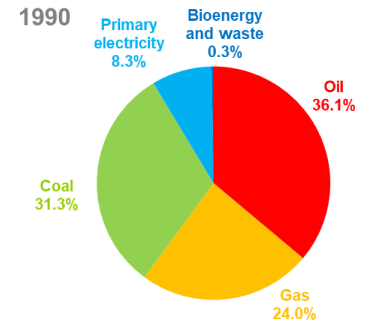
\includegraphics[height=5cm]{assets/graphs/energy-consumption_1990.png}
    \end{subfigure}
    \begin{subfigure}{0.40\textwidth}
    \centering
    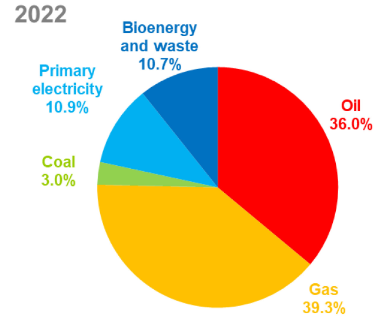
\includegraphics[height=5cm]{assets/graphs/energy-consumption_2022.png}
    \end{subfigure}
\caption{Total energy production in the United Kingdom in 1990 and 2022 \cite{departmentforenergysecurityandnetzero2023UKEnergyBrief}.}
\label{fig:fuel-consump}
\end{figure}

The growth of international populations and industry have meant that the global market for energy is higher than ever \cite{newell2019GlobalEnergyOutlook} and the reliance on fossil fuels is ubiquitous despite international efforts to quell the emission of carbon into the atmosphere \cite{unitednations2015ParisAgreementUNFCCC}. Nevertheless, with the price of green energy at its lowest historical levels \cite{internationalrenewableenergyagency2022RenewablePowerGeneration} and the threat of irreversible climate crises imminent, work must be done to adopt renewable energy sources. In Britain, the removal of coal as an energy source was successful, as shown in \fig{fig:fuel-consump}. This \emph{fuel switching} from coal to gas and oil, promoted by effective economic factors, led to a 6\% decrease in the country's overall carbon emissions \cite{wilson2018RapidFuelSwitching}. With gas, methane is almost exclusively burnt, and the domestic and industrial sectors account for approximately a third each (237 TWh and 206 TWh of methane, respectively) of the total methane consumption in Britain in 2023 \cite{departmentforenergysecurityandnetzero2023HistoricalGasData}.

One appropriate renewable source of energy is that of hydrogen, which is unlikely to replace the usage of fossil fuels but may be used alongside gas in applications where this gas was already being burnt \cite{momirlan2005PropertiesHydrogenFuel}. Although greener than gas or oil, different hydrogen production processes \cite{dasilvaveras2017HydrogenTrendsProduction} cause significant variations in carbon emissions \cite{nationalgrid2022HeatingOurHomes}. Hydrogen represents an attractive energy source \cite{momirlan2005PropertiesHydrogenFuel}, particularly through fuel cells \cite{momirlan2005PropertiesHydrogenFuel} and combustion \cite{lanz2001ModuleHydrogenUse, stepien2021ComprehensiveOverviewHydrogenFueled}. The combustion of hydrogen in particular may be used for internal combustion engines, gas turbines cookers and gas boilers \cite{momirlan2005PropertiesHydrogenFuel}. It has also been estimated that by 2040, the demand for hydrogen in the United States will have grown to 15 million tons \cite{molkov2007HydrogenSafetyResearch} and represents the growth of the \emph{hydrogen economy}.

Hydrogen presents significant safety concerns \cite{green2006HydrogenSafetyIssues} especially in its gaseous form, with an obvious example of this being the 1937 Hindenburg disaster \cite{dilisi2017HindenburgDisasterCombining}. One probable cause being the light H\sub{2} molecules escaping the Zeppelin and catching alight. This property of hydrogen is the primary cause of concern in premixed, hydrogen-deficient (lean) combustion regimes, where the \emph{thermodiffusive instability} dominates. Premixed combustion, where the reactants enter the combustor already mixed, is the dominant regime for combustion in engineering applications due to the higher heat released compared to non-premixed flames. In this report, we focus on premixed combustion instabilities, especially the \emph{hydrodynamic instability} phenomena which is experienced purely as a result of the thermal expansion of gas in a premixed flame \cite{matalon2018DarrieusLandauInstability}. The \emph{thermoacoustic instabilities} of premixed flames are also covered, which are known to cause significant damage to combustors as a result of a coupling between the acoustics of the flame and combustor \cite{morgans2024ThermoacousticInstabilityCombustors}. Thermoacoustic instabilities will be the primary focus of this PhD in the future.

Of particular interest are how these fuels behave in complex geometries, especially for the purposes of porous media combustion (PMC). The benefits and applications of PMC are wide-reaching: PMC enables more effective transfer of heat from the combustion reaction to combustor \cite{mujeebu2009CombustionPorousMedia}; hydrogen combustion in PMCs enable leaner combustion \cite{tseng2002EffectsHydrogenAddition}; PMC has been used on the smallest scales, including in micro thermophotovoltaic systems \cite{pan2015HydrogenOxygenPremixed}; and PMC has been used for the passive control of the aforementioned thermoacoustic instabilities \cite{meadows2015PorousInsertsPassive, dowd2018ThermoacousticInstabilityModel}. Analytic studies form the foundation of instability research and provide many predictions for flames in simple geometries, but fall short in the case of these complex geometries. The next tool in our tool belt is Direct Numerical Simulation (DNS) \cite{orszag1970AnalyticalTheoriesTurbulence}, where the fluid is fully resolved.

The main objectives of this report are to perform a holistic literature review of relevant work and to show evidence of initial findings related to the PhD topic. \chap{ch:background} presents the governing combustion equations and present simplifications which can be made to formulate a simpler, mathematically tractable system of equations. On top of this, the Rankine-Hugoniot jump conditions and method of lines are presented as prerequisite knowledge for the coming chapters. This is followed by \chap{ch:lit_review} which constitutes the plurality of the report's contents and provides a literature review of the theoretical and experimental studies into the thermodiffusive, hydrodynamic and thermoacoustic premixed combustion instabilities. Initial findings are then given in \chap{ch:orig_work}, where we use a mesh-free combustion DNS code developed in \cite{king2022HighorderSimulationsIsothermal, king2024MeshfreeFrameworkHighorder, king2020HighOrderDifference, king2024SunsetFlamesDNSCode} to simulate hydrodynamically unstable flames in a simple periodic geometry. This is compared against the hydrodynamic theory of flames covered in \chap{ch:lit_review} and in particular to the Michelson-Sivashinsky equation which predates this theory. A spectral solver for the Michelson-Sivashinsky equation is also developed, but is found to be insufficient in the case of high heat releases and negligible tangential velocities. Finally, conclusions relating to this report are drawn in \chap{ch:conc} and \chap{ch:plan} organises a plan for the work proceeding this report.




